\documentclass[aspectratio=169]{beamer} % Aspectratio is to change the format and 169 is for 16:9
\usepackage[utf8x]{inputenc}
\usepackage[francais]{babel}
\usepackage{graphicx} % Allows including images
\usepackage{booktabs} % Allows the use of \toprule, \midrule and \bottomrule in tables
%\usepackage[T1]{fontenc}

% ajout des librairie pour l'insertion de code
\usepackage{xcolor}
\usepackage{listings}
\lstset{
	basicstyle=\ttfamily,
	stringstyle=\ttfamily\color{green!50!black},
	keywordstyle=\color{blue}\bfseries,
	commentstyle=\color{red!50!black}\itshape,
	showstringspaces=true,
	tabsize=2, frame=single,
	numbers=left, numberstyle=\tiny,
	firstnumber=1, stepnumber=1, numbersep=5pt, breaklines=true
}

\mode<presentation> {
	
	% The Beamer class comes with a number of default slide themes
	% which change the colors and layouts of slides. Below this is a list
	% of all the themes, uncomment each in turn to see what they look like.
	
	%\usetheme{default}
	%\usetheme{AnnArbor}
	%\usetheme{Antibes}
	%\usetheme{Bergen}
	%\usetheme{Berkeley}
	%\usetheme{Berlin}
	%\usetheme{Boadilla}
	\usetheme{CambridgeUS}
	%\usetheme{Copenhagen}
	%\usetheme{Darmstadt}
	%\usetheme{Dresden}
	%\usetheme{Frankfurt}
	%\usetheme{Goettingen}
	%\usetheme{Hannover}
	%\usetheme{Ilmenau}
	%\usetheme{JuanLesPins}
	%\usetheme{Luebeck}
	%\usetheme{Madrid}
	%\usetheme{Malmoe}
	%\usetheme{Marburg}
	%\usetheme{Montpellier}
	%\usetheme{PaloAlto}
	%\usetheme{Pittsburgh}
	%\usetheme{Rochester}
	%\usetheme{Singapore}
	%\usetheme{Szeged}
	%\usetheme{Warsaw}
	
	% As well as themes, the Beamer class has a number of color themes
	% for any slide theme. Uncomment each of these in turn to see how it
	% changes the colors of your current slide theme.
	
	%\usecolortheme{albatross}
	%\usecolortheme{beaver}
	%\usecolortheme{beetle}
	%\usecolortheme{crane}
	%\usecolortheme{dolphin}
	%\usecolortheme{dove}
	%\usecolortheme{fly}
	%\usecolortheme{lily}
	%\usecolortheme{orchid}
	%\usecolortheme{rose}
	%\usecolortheme{seagull}
	%\usecolortheme{seahorse}
	%\usecolortheme{whale}
	%\usecolortheme{wolverine}
	
	%\setbeamertemplate{footline} % To remove the footer line in all slides uncomment this line
	%\setbeamertemplate{footline}[page number] % To replace the footer line in all slides with a simple slide count uncomment this line
	
	%\setbeamertemplate{navigation symbols}{} % To remove the navigation symbols from the bottom of all slides uncomment this line
}

%----------------------------------------------------------------------------------------
%	TITLE PAGE
%----------------------------------------------------------------------------------------

\title[Cube LED]{Cube à LED} % The short title appears at the bottom of every slide, the full title is only on the title page

\author{Alan Devaud \& Kevin Amado \& Gregory Mendez}
\institute[CFPT] 
{
	Centre de Formations Professionnelle Technique \\
	Ecole d'informatique \\ 
	\medskip
	\textit{Travail de semestre Technicien 1\up{er} et 2\up{ème}}
}
\date{\today}


\begin{document}
	
	\begin{frame}
		\titlepage
	\end{frame}
	
	\begin{frame}
		\frametitle{Sommaire} 
		\tableofcontents % Throughout your presentation, if you choose to use \section{} and \subsection{} commands, these will automatically be %printed on this slide as an overview of your presentation
	\end{frame}
	
	%----------------------------------------------------------------------------------------
	%	PRESENTATION SLIDE
	%----------------------------------------------------------------------------------------
	
	
	% Introduction
	\section{Introduction}
	\begin{frame}
		\frametitle{Introduction}
		\begin{columns}[c]
			\column{.5\textwidth}
			\begin{itemize}
				\item Application pour controler un cube à LED
				\item Reprise d'un ancien projet
				\item Projet en groupe
				\item Association technicien 1\up{er} et 2\up{ème}
				\item Temps à disposition 48 périodes
			\end{itemize}
		
			\column{.5\textwidth}
			\begin{figure}[htp]
				\centering
				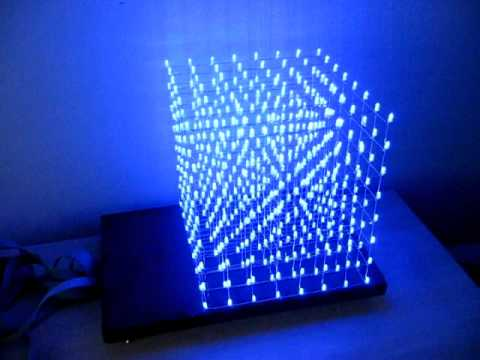
\includegraphics[width=5cm]{Img/cube.jpg}
			\end{figure}
		\end{columns}
	\end{frame}
	
	
	%Méthode mise en oeuvre
	\section{Matériels}
	\begin{frame}
		\frametitle{Matériels}
		\begin{columns}[c]
			\column{.5\textwidth}
			\begin{itemize}
				\item Cube à LED
				\item 512 LED (8x8x8)
				\item Deux versions à disposition
			\end{itemize}
			
			\column{.5\textwidth}
			\begin{itemize}
				\item Visual Studio 2013
				\item Windows form C\#
				\item Monogame
			\end{itemize}
			
			
		\end{columns}
	\end{frame}
	
	\section{Objectifs}
	\begin{frame}
		\frametitle{Objectifs}
		\begin{columns}[c]
			\column{.45\textwidth}
			\begin{itemize}
				\item Application windows
				\item Gérer les LEDs du cube
				\item Communication par USB
 				\item Visualisation 3D d'un cube
			\end{itemize}
			
			\column{.55\textwidth}
			\begin{figure}
				\centering
				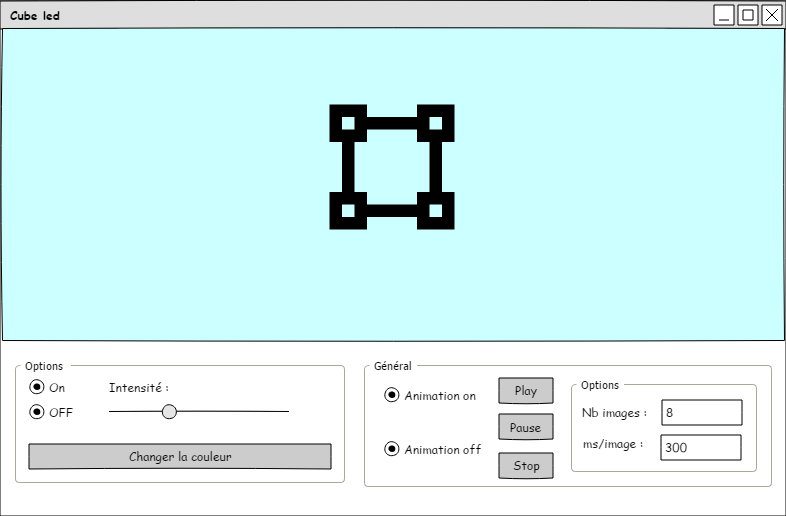
\includegraphics[width=7cm]{Img/windform.png}
			\end{figure}
		\end{columns}
	\end{frame}
	
	\section{Annalyse fonctionnel}
	\subsection{Communication}
	\begin{frame}
		\frametitle{Communication}
		\begin{columns}[c]
			\column{.5\textwidth}
			\begin{itemize}
				\item Communication par USB
				\item Utilisation d'une bibliothèque
				\item Création d'une sur-couche à la bibliothèque
				\item Convertit les données au bon format du cube
			\end{itemize}
			
			\column{.5\textwidth}	
			\begin{itemize}
				\item Données reçues : \emph{data[x][y][z] = Frame;State;Intensity;Color;}
				\item Données à envoyer : \emph{data[x][y][frame] = (0 - 256)}
			\end{itemize}
			
		\end{columns}
	\end{frame}

	\subsection{Visualisateur 3D}
	\begin{frame}
		\frametitle{Visualisateur 3D}
		\begin{columns}[c]
			\column{.5\textwidth}
			\begin{itemize}
				\item Monogame est une bibliothèque qui implémente XNA
				\item Création d'une sphere 3D à l'aide d'une classe source 
				\item Intégration du projet monogame dans un projet windows form
				\item picking
			\end{itemize}
			
			\column{.5\textwidth}	
			\begin{itemize}[htp]
				\centering
				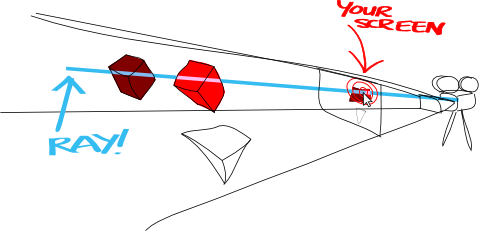
\includegraphics[width=6cm]{Img/ray.png}
			\end{itemize}
		
		\end{columns}
	\end{frame}

	\subsection{Diagramme de classe}
	\begin{frame}
		\frametitle{Diagramme de classe}
		\begin{figure}[htp]
			\centering
			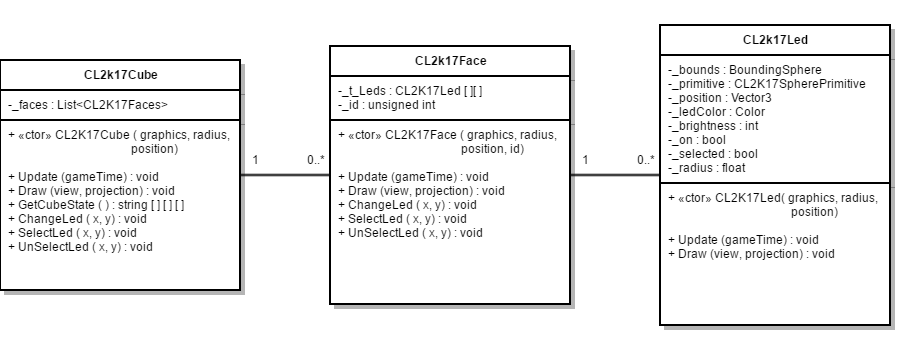
\includegraphics[width=14cm]{Img/DiagrammeUmlCube.png}
		\end{figure}
	\end{frame}

	
	
	\section{Démonstration}
	\begin{frame}
		\frametitle{Démonstration}
		\begin{figure}
			\centering
			
\includegraphics[width=5cm]{Img/demo.jpg}
		\end{figure}
	\end{frame}

	\section{Améliorations}
	\begin{frame}
		\frametitle{Améliorations}
		\begin{columns}[c]
			\column{.5\textwidth}
			\begin{itemize}
				\item Picking
				\item Possibilité des animations
				\item Modification en temps réel du cube à LEDs
			\end{itemize}
		
			\column{.5\textwidth}
			\begin{figure}
				\centering
				
\includegraphics[width=3cm]{Img/upgrade.png}
			\end{figure}
		\end{columns}
	\end{frame}
	
	\section{Conclusion}
	\begin{frame}
		\frametitle{Conclusion}
		\begin{columns}[c]
			\column{.55\textwidth}
			\begin{itemize}
				\item Utilisation de\emph{Monogame} dans une \emph{winform}
				\item Picking et ses difficultés
				\item Utilisation d'un cube à LED
			\end{itemize}
			
			\column{.45\textwidth}
			\begin{itemize}
				\item Communication par USB
				\item Création de bibliothèque
				\item Bon projet
			\end{itemize}
		\end{columns}
		
	\end{frame}
	
	\section{Questions}
	\begin{frame}
		\begin{figure}
			\centering
			
\includegraphics[width=.9\textwidth]{Img/question.jpg}
		\end{figure}
	\end{frame}
\end{document} 